\section{\bf \our Step 2: TX Locations' Distributions to Precise Locations}
\label{sec:detect}

In this section, we present the second step of our overall localization approach. We refer to
this step as the {\em peak detection} step, as the goal is to detect the peaks within the 
Gaussian distributions in the input image (which is also the output image of the first step).
%%%%
The first step outputs an image that has multiple distributions (presumably, Gaussian), whose
peaks need to be interpreted as precise locations of the transmitters/intruders.
%%%%%%%%%%%%
As, our end goal is to determine the precise locations of the present transmitters, we develop techniques to detect peaks within  the output image of the first step. 
%%%%%%%%%%%%%%%%%%%%%%%
We propose two different strategies for the peak-detection task. The first strategy is a straightforward peak detection algorithm based on finding local maximal values, while the 
second strategy is based on framing the problem as an object detection task; for the second strategy, we utilize a widely used state-of-the-art computer vision model called YOLOv3~\cite{yolov3}.

\para{Simple Peak Detection Method.}
The simple and straightforward peak detection method is to designate pixels with
locally maximal values as peaks, subject to certain thresholds.
%%%%%%%%%
More formally, we use a threshold $x$ for a peak value, and also use a parameter $r$ to define a $r$-radius neighborhood of a pixel. 
Then, any pixel whose value is more than $x$ and is the maximum among all pixels with a $r$-radius neighborhood, is designated as a peak (transmitter location). 
We use $x=2$ and $r=3$, in our evaluations.
%%%%%%%%%%%%%
Note that each pixel represents a subarea; thus, a pixel designated as pixel only 
implies the transmitter location at the {\em center} of the corresponding subarea.
%%%%%%%
To localize the transmission more precisely with the pixel's subarea, we use a scheme that localizes the transmitter within the subarea by computing a weighted average of the peak pixel's coordinate and the peak's neighbor pixels' coordinates.
The weight of a pixel is the predicted pixel value itself from the first step \imgimg.
%%%%%%%%%%%%%%%%%%%%%
We refer to the above simple approach for the second-step of \our as \simpeak.

\begin{figure}
	\centering
	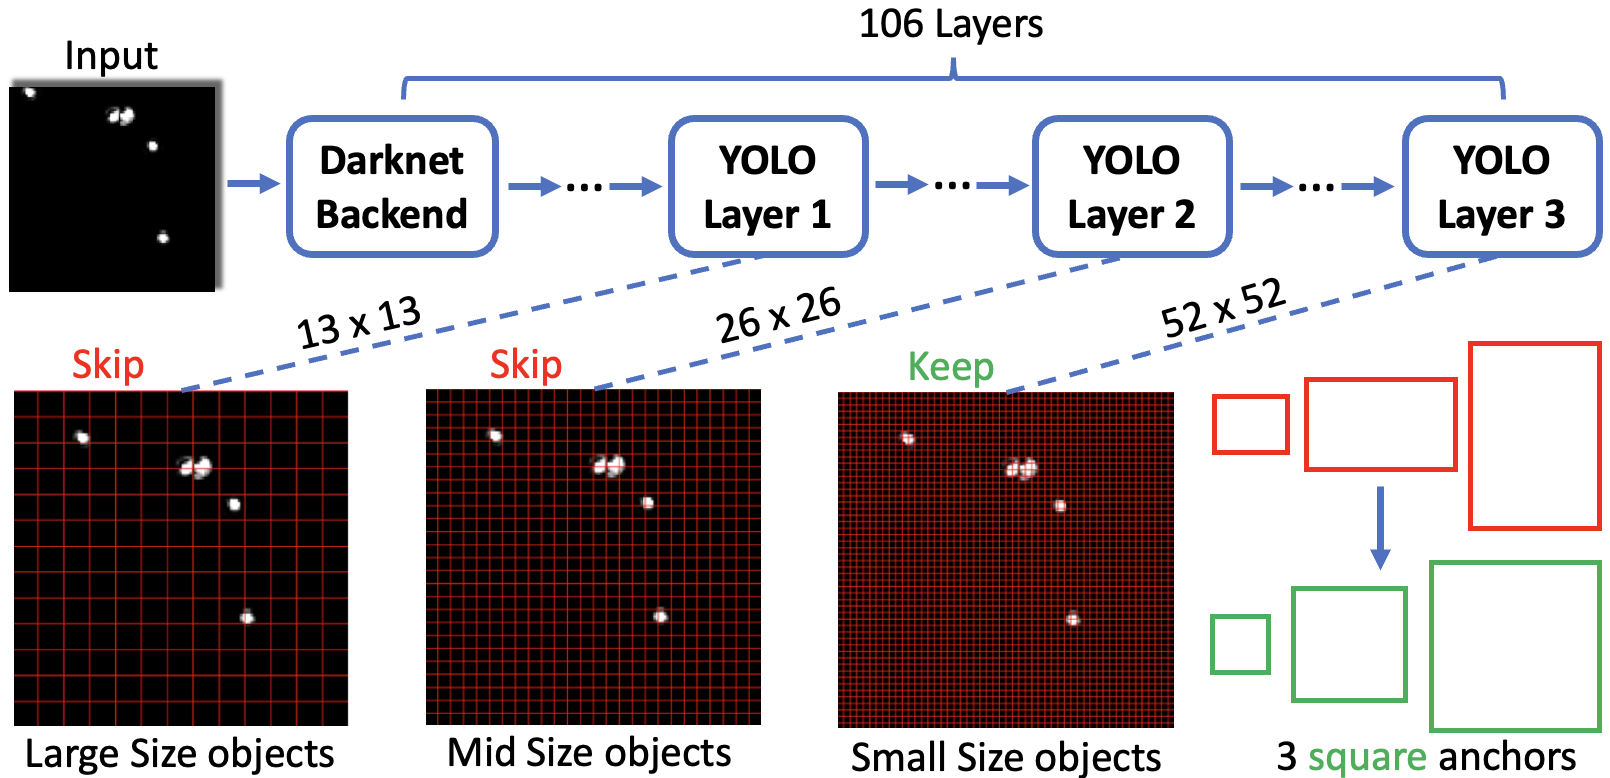
\includegraphics[width=0.75\textwidth]{chapters/wowmom-pmc/figures/yolo.png}
	\vspace{-0.1in}
	\caption{Our \yolocust in the second step of the \our. The two major customization are: (i) Use only the third YOLO layer that detects small size objects (the output of \yolocust is the bounding box predicted by the third YOLO layer and we use the center of the bounding box as the transmitter location), and (ii) change the rectangle anchors to square anchors.}
	\label{fig:yolo}
\end{figure}

\subsection{\bf Object-Detection Based Precise Localization: \yolocust} 

The simple hand-crafted method described in the previous subsection performs reasonable well in most cases in our simulations. 
However, its key drawback is that it needs appropriate threshold values that may vary from case to case; such thresholds can be difficult to determine, especially since
the input images (with distributions) are not expected to be perfect as they are themselves output of a learning model.
Inaccurate threshold values can lead to false alarms and misses. 
Also, the previous method is not sufficiently accurate at the sub-pixel level, where
each pixel may represent a large area such as $10m \times 10m$ or even $100m \times 100m$. Thus,
we propose a CNN-based learning method that overcomes the above shortcomings.  
CNN has been widely used for object detection in different areas~\cite{objectdetectionsurvey,alizadeh21}.

We frame this problem as an object detection task where the objective is to detect and localize
known objects in a given image. We observe that our second-step peak detection problem is essentially an object detection problem where the ``object" to detect is a ``peak".
Thus, we turn the \mtl problem of localizing multiple transmitters into detecting 
peaks in the images output by \imgimg model. 
For object/peak detection, we design \yolocust, our customized version of YOLOv3~\cite{yolov3}.
Fig.~\ref{fig:peaks} is a zoom-in of localizing two close by transmitters (peaks) in Fig.~\ref{fig:overall}(b).

\softpara{Peak Detection Using \yolocust.} 
Object detectors are usually comprised of two parts: (i) a backbone which is usually pre-trained on ImageNet, and (ii) a front part (head), which is used to predict bounding boxes of objects, probability of an object present, and the  object class. 
For the front part, object detectors are usually classified into two categories, i.e., one-stage detectors such as the YOLO~\cite{cvpr16-yolo} series, and two-stage detectors such as the R-CNN~\cite{cvpr14-rcnn} series.
We choose the one-stage YOLO series because of its computational efficiency, high popularity and available ways to customize it for our specific context. We refer to the customized version as \yolocust, see Fig.~\ref{fig:yolo}.
%%%%%%%%%
Implementing a 106-layer deep neural network with a complex design from scratch is
out of scope of our work. 
Thus, we use a publicly available source repository~\cite{yolo-github} and made customization on top of it.
We refer to the architecture that uses \imgimg $\ $and \yolocust in sequence as \our, our key product.  
In addition, we use \imgimg in combination with the uncustomized original YOLOv3,
and refer to it as \ouryolo (still change the class number to one).
%\blue{For the two important hyper-parameters of YOLOv3, object confidence threshold and intersect-of-union threshold for non-maximum suppression, we tweaked to 0.8 and 0.5 respectively.}

\softpara{Customization of YOLOv3}.
Overall, we incorporated four customization to YOLOv3, of which two are significant and the
other two are relatively minor. See Table~\ref{table:yolocust}. YOLOv3 is designed to be a general object detector that can detect objects of various sizes, shapes, and classes within input images
of various sizes. However, in our context, the input images are of a fixed size, with
only a single class of objects which are relatively small and semi-circular. 
Based on the above observations, we make changes to the original YOLOv3 that both 
decrease the model complexity and improve its performance.

\begin{figure}[t]
	\centering
	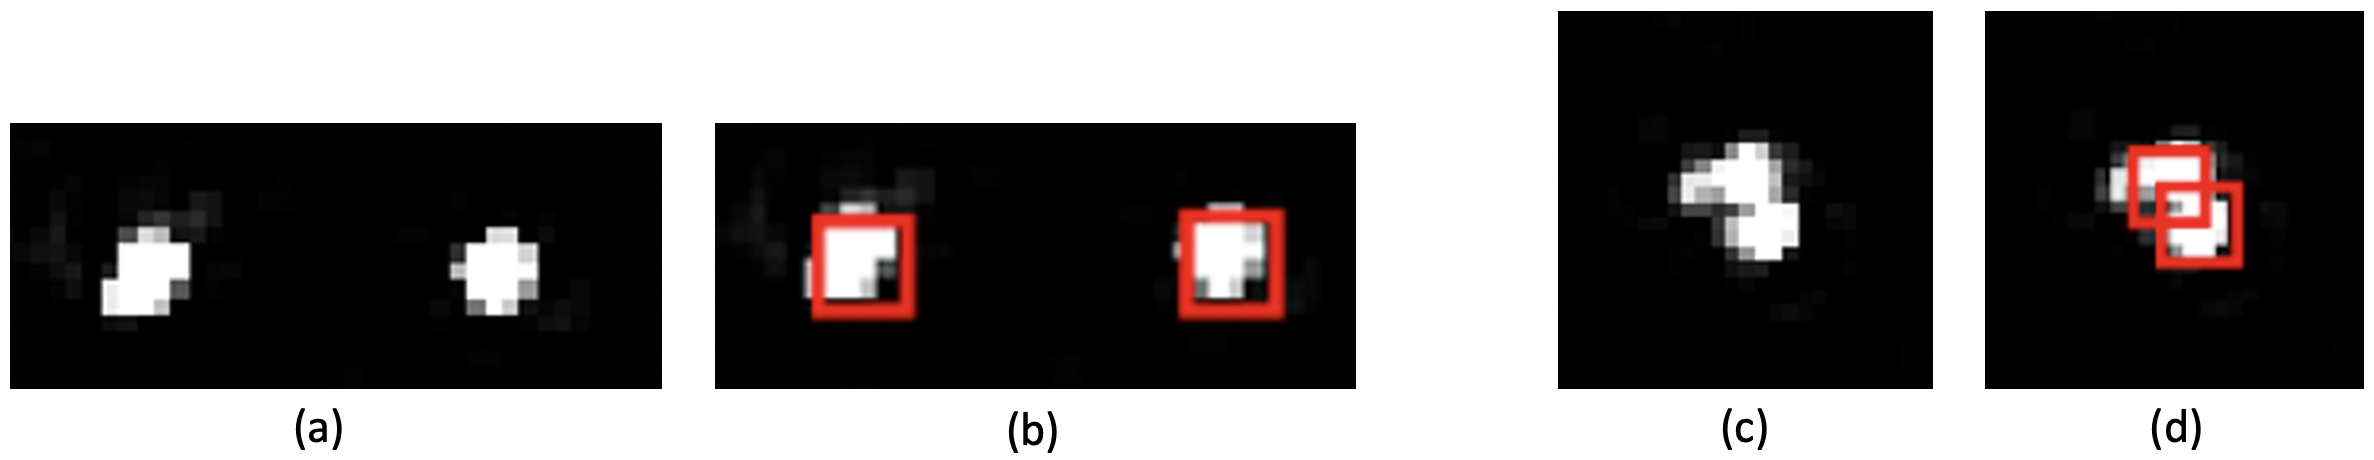
\includegraphics[width=0.75\textwidth]{chapters/wowmom-pmc/figures/peaks.png}
	\vspace{-0.1in}
	\caption{(a) is the zoom-in of two peaks at the bottom of the Fig.~\ref{fig:overall} example.
	(c) is the zoom-in of the two close by peaks in the middle right of the Fig.~\ref{fig:overall} example. (b) and (d) shows the bounding boxes that \yolocust outputs for (a) and (c) respectively.}
	\label{fig:peaks}
\end{figure}

\begin{table}[t]
    \caption{Differences between the original YOLOv3 and our \yolocust.}
    \centering
    \begin{tabular}{ |p{6cm}|p{6cm}| } 
     \hline
     YOLOv3 & \yolocust  \\
     \hline \hline
     Has three YOLO layers at $13\times13$, $26\times26$, and $52\times52$ for detection & Only use the last $52\times52$ YOLO layer for detection (skip the first two YOLO layers) \\
     \hline
     Has 3 different rectangle anchors for each YOLO layer & Has 3 square anchors \\
     \hline
     Every 10 batches, randomly chooses a new input image dimension size & Do not randomly choose new input dimension size \\ 
     \hline
     Has 80 different categories of object class & Only has one category for the peak class \\ 
     \hline
    \end{tabular}
    \label{table:yolocust}
\end{table}

{\em Customization Details}. 
The first and second changes presented in Table~\ref{table:yolocust} are major changes and we elaborate them in the following paragraphs.
%%%%%%%%o
Making prediction at three different scales is one of the highlights of YOLOv3 and an improvement comparing to the previous version YOLOv2 which was prone to missing at detecting small objects. 
As shown in Fig.~\ref{fig:yolo}, the coarse-grain $13\times13$ YOLO layer-1 is designed for detecting large size objects, 
the $26\times 26$ YOLO layer-2 is designed for detecting middle-sized objects, and 
the fine-grained $52\times52$ YOLO layer-3 is designed for detecting small-sized objects.
Since the peaks in our translated images are always small objects, we only use the last $52\times 52$ YOLO 
detection layer (and skip the first two YOLO layers).
%%%%%%%
As shown in Fig.~\ref{fig:yolo}, by ``skipping" the two YOLO layers means that we do not use them in 
computing the overall loss function and their outputs are not used in predicting the bounding boxes.
%\red{``Skip'' shown in Fig.~\ref{fig:yolo} is implemented as the first two YOLO layers are not calculated in the overall loss function and their outputs are not used for predicting bounding boxes.}
% Thus, the loss function depends only on the last 52x52 YOLO layer-3, instead of all three YOLO layers and the optimization process targets only the  the last 52x52 YOLO layer.
% \red{The above results in less parameter values to be learnt via training, and thus, reduces the training cost 
% substantially. }
%%%%%%%%%%%%%%%%%%
In our \yolocust, the only YOLO layer predicts 8112 bounding boxes, since it has a 
dimension of $52\times 52$ and each cell results in prediction of 3 bounding boxes; this is in contrast
to the original YOLOv3, which predicts 10647 bounding boxes ($3 \times (13\times13 + 26\times26 + 52\times52) = 10647$).

The anchor box is one of the most important hyperparameters of YOLOv3 that can be tuned to improve
its performance on a given dataset.  The original YOLO's anchor boxes are $10\times13$,  $16\times30$, and $33\times23$ (for
the input image of size $416\times416$ pixels), which are essentially bounding boxes of a rectangular shape. 
%%%%%%%%%%%%%
These original YOLOv3 anchors were designed for the Microsoft COCO \cite{mscoco} data set, and were chosen
since they best describe the dimensions of the real world objects in the MS COCO data set. In our context,
since the peaks are generally squares---we use the anchor boxes to be $15\times15$, $25\times25$, and $35\times35$.

%%%%%%%%%%% peaks %%%%%%%%%

\softpara{Input Image for \yolocust.}
The first step \imgimg's output image is $100\times100$, while the second step \yolocust's input is required\footnote{YOLOv3 was developed before our work and the YOLOv3 authors set the input size of the CNN model to $3\times416\times416$.~Although we are customizing their YOLOv3 model, we cannot change the input size because changing it will change the convolutional layer structure, which will 
preclude us from using the pre-trained weights in the YOLOv3 backbone.} 
to be a three-channel (RGB) image with each channel being size of $416\times 416$. 
%%%%%%%%%%%
To feed the output of \imgimg to \yolocust, we do the following: (i) First, we duplicate 
the \imgimg's output image to create two more copies and thus create a three-channel image
of 100 $\times$ 100 size channels; (ii) Next, we resize the $100\times100$ channels to $416\times416$ channels using the PyTorch's default ``nearest neighbor" interpolation. See Fig.~\ref{fig:yolo-preprocess}.

\softpara{Output of \yolocust.}
YOLO treats objected detection as a regression problem. The regression target (or ``label") for an object is a five-value tuple $(x, y,$ $length,$ $width, class)$. 
In our case, there is only one $class$. 
$x$ and $y$ are real number location coordinates of the center of the bounding box, which we use as the location of the transmitter. 
$Width$ and $height$ determine the size and shape of the object---which we consistently set to be 5 each to signify a $5\times5$ square. 
Note that the center of the bounding box is in the continuous domain. 
Thus, we are able to get sub-pixel level location of the transmitters.


\begin{figure}[t]
	\centering
	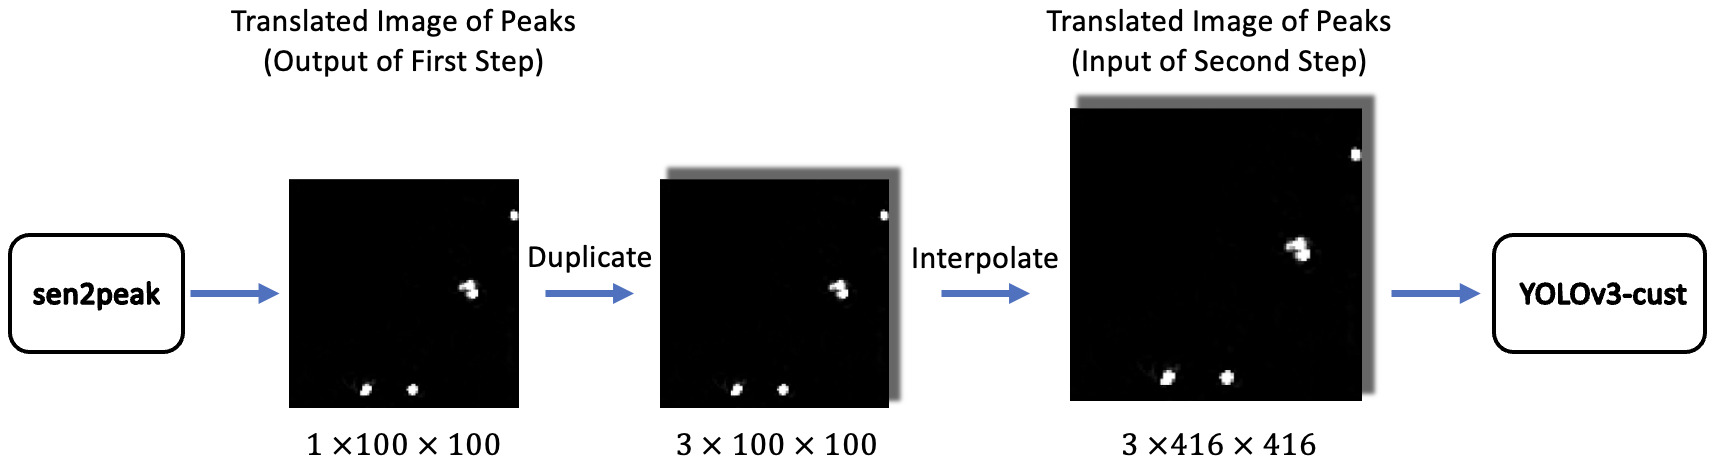
\includegraphics[width=0.9\textwidth]{chapters/wowmom-pmc/figures/yolo-preprocess.png}
	\vspace{-0.1in}
	\caption{The data processing of \imgimg's output to get \yolocust's input of correct size.}
	\label{fig:yolo-preprocess}
\end{figure}


%\blue{Labeling the training dataset of \yolocust is important. Given the output of the first step's \imgimg and the ground truth of the TX locations, we label the Gaussian peaks as a class peak who has a value higher than 0.3 at the ground truth's pixel location (recall in \ref{subsec:imgimg_output_image} that the peak at the target representation of a TX in \imgimg is 10). That is to say, when \imgimg outputs a very low altitude Gaussian distribution (i.e. near flat) for a transmitter, that near flat area will not be labeled as a peak for the training data of \yolocust.}


%In summary, we customized both the number of YOLO layers and anchor box configurations, to decrease the model complexity and increase accuracy for our context. The increase of accuracy of our system is demonstrated in the next section.
